\chapter{Metodi Agili}
I \textbf{metodi agili} sono stati definiti per rispondere all'esigenza di dover
affrontare lo sviluppo di software in continuo cambiamento, quindi saranno dei 
processi di gestione dello sviluppo che si addattano facilmente al cambiamento. 
Durante lo sviluppo si hanno vari passaggi:
\begin{itemize}
      \item Comprensione dei prerequisiti.
      \item Scoperta di nuovi requisiti o cambiamento dei vecchi.
\end{itemize}

Questa situazione rendeva difficile lo sviluppo secondo il vecchio metodo
waterfall portando al fallimento di diversi progetti.

I metodi agili ammettono che i requisiti cambino in modo “naturale” durante il
processo di sviluppo software e per questo assumono un modello di processo
circolare, con iterazioni della durata di un paio di settimane (\ref{fig:agili}).

\begin{figure}[!ht]
      \centering
      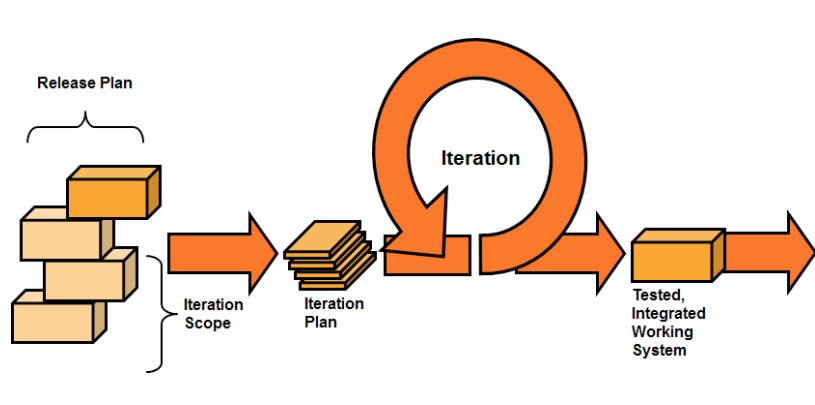
\includegraphics[scale=0.5]{img/agili/agili.png}
      \caption{Rappresentazione grafica di un metodo agilie.}
      \label{fig:agili}
\end{figure}

Potenzialmente dopo un'iterazione si può arrivare ad un prodotto che può essere
messo in produzione. Dopo ogni rilascio si raccolgono feedback per poter rivalutare
i requisiti e migliorare il progetto. Si hanno quindi aspetti comuni nei metodi agili e nel loro processo:
\begin{itemize}
      \item \textit{Enfasi sul team}, sulla sua qualità e sulla sua selezione.
      \item Il \textit{team è self organizing}, si da importanza ai vari membri
            del team dato che non esiste un manager ma è il team stesso a gestire lo sviluppo.
      \item \textit{Enfasi al pragmatismo}, focalizzandosi su una documentazione
            efficace evitando di produrre documenti inutili e difficili da mantenere.
      \item \textit{Enfasi sulla comunicazione diretta}, sostituendo i documenti
            suddetti con meeting e riunioni periodiche.
      \item \textit{Enfasi sull'idea che nulla sia definitivo}: la perfezione non
            deve essere seguita fin da subito ma saranno gli step a portare al raggiungimento
            di una perfezione finale.
      \item \textit{Enfasi sul controllo costante} della qualità del prodotto,
          anche tramite:
            \begin{itemize}
                  \item \textbf{Continuous testing} grazie al quale un insieme di test viene
                        eseguito in modo automatico dopo ogni modifica.
                  \item \textbf{Analisi statica} e dinamica del codice al fine di trovare
                        difetti nello stesso.
                  \item \textbf{Refactoring}.
            \end{itemize}
\end{itemize}

I metodi agili sono molto “elastici” e permettono la facile definizione di nuovi
metodi facilmente adattabili al singolo progetto.
\section{Scrum}
Uno dei più famosi, tra i vari metodi agili, è \textbf{scrum} (\ref{fig:scrum}).

\begin{figure}[!ht]
      \centering
      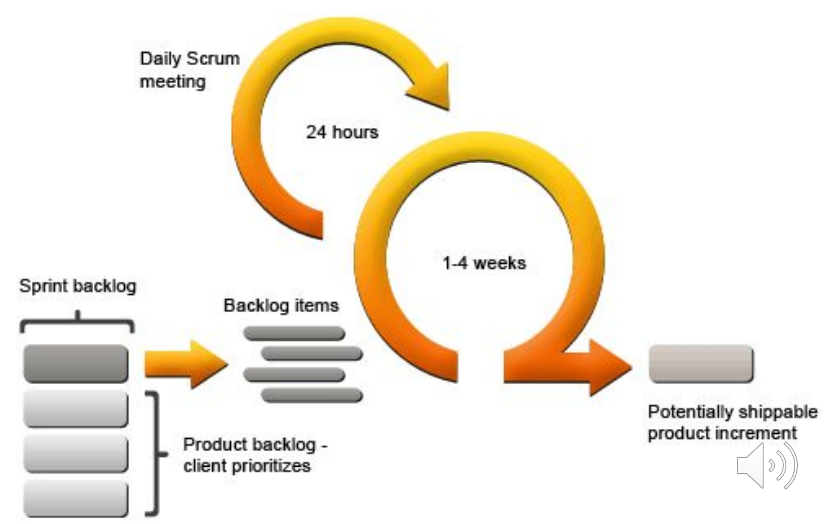
\includegraphics[scale=0.5]{img/agili/scrum.png}
      \caption{Rappresentazione grafica del processo scrum}
      \label{fig:scrum}
\end{figure}
In questo caso la parte di sviluppo e iterazione prende il nome di \textbf{sprint}
ed ha una durata variabile tra una e quattro settimane, per avere un rilascio
frequente e una veloce raccolta di feedback. I requisiti sono raccolti nel cosiddetto
\textbf{product backlog}, con priorità basata sulla base delle indicazioni del
committente. Ad ogni sprint si estrae dal product backlog lo \textbf{sprint backlog},
ovvero il requisito (o i requisiti) da implementare nello sprint. Lo sprint backlog
viene analizzato nel dettaglio producendo i vari \textbf{backlog items}, ovvero
le singole funzionalità che verranno implementate nello sprint. Si ottiene quindi
di volta in volta un pezzo di prodotto finale, testato e documentato. Durante le
settimane di sprint si effettua anche un meeting giornaliero utile per mantenere
alti i livelli di comunicazione e visibilità dello sviluppo. Durante il meeting
ogni sviluppatore risponde a tre domande:
\begin{enumerate}
      \item Cosa è stato fatto dall'ultimo meeting?
      \item Cosa farai fino al prossimo meeting?
      \item Quali sono le difficoltà incontrate?
\end{enumerate}

L’ultimo punto permette la cooperazione tra team members, consci di cosa ciascuno
stia facendo. Durante il processo scrum si hanno quindi tre ruoli:
\begin{enumerate}
      \item Il \textbf{product owner}, il committente che partecipa tramite feedback
            e definizione dei requisiti.
      \item Il \textbf{team} che sviluppa.
      \item Lo \textbf{scrum master} che controlla la correttezza di svolgimento
            del processo scrum.
\end{enumerate}

Lo scrum master interagisce in ogni fase, fase che viene comunque guidata tramite
meeting:
\begin{itemize}
      \item \textbf{Sprint planning meeting}, ad inizio sprint per pianificare 
            cosa fare nello sprint
      \item \textbf{Daily scrum meeting}, il meeting giornaliero per aggiornare
            tutti i membri del team su quello che ciascuno sta facendo e deve essere
            il più breve possibile
      \item \textbf{Sprint review meeting}, in uscita dallo sprint per lo studio dei
            risultati e analisi di quello che è stato sviluppato
      \item \textbf{Sprint retrospective meeting}, in uscita dallo sprint per lo
            studio, tra i membri del team, di eventuali miglioramenti da apportare 
            al processo Scrum e allo sviluppo del prodotto.
\end{itemize}

Spesso nelle singole iterazioni si utilizza la metodologia di sviluppo basata
sull'\textbf{extreme programming}, ovvero:
\begin{itemize}
	\item planning delle attività
	\item short release
	\item simple design
	\item refactoring
	\item Test first design
	\item Pair programming
	\item Collective Ownership
	\item Continuous Integration
	\item 40-h week
	\item On-site customer
	\item coding standard
	\item Open workspace
\end{itemize}

\section{Extreme Programming}
Un altro tipo di metodo agile è l'\textbf{extreme programming}, ormai poco usato.
I requisiti prendono i nomi di stories, delle narrazioni in cui l’attore
(futuro utente del sistema) cerca di svolgere un compito. Vengono scelti quindi stories
per la prossima iterazione, dove si hanno testing e revisione continua. Le release
di ogni iterazione vengono catalogate per importanza (con anche la solita 
collezione di feedback).